\documentclass[DIN, pagenumber=false, fontsize=11pt, parskip=half]{scrartcl}

\usepackage{amsmath}
\usepackage{amsfonts}
\usepackage{amssymb}
\usepackage{enumitem}
\usepackage[utf8]{inputenc} % this is needed for umlauts
\usepackage[T1]{fontenc} 
\usepackage{commath}
\usepackage{xcolor}
\usepackage{booktabs}
\usepackage{float}
\usepackage{tikz-timing}
\usepackage{tikz}
\usepackage{multirow}
\usepackage{colortbl}
\usepackage{xstring}
\usepackage{circuitikz}
\usepackage{listings} % needed for the inclusion of source code
\usepackage[final]{pdfpages}
\usepackage{subcaption}
\usepackage{import}
\usepackage{bm}
\usepackage{hyperref}
\usepackage{todonotes}

\usetikzlibrary{calc,shapes.multipart,chains,arrows,shadows}

\newcommand*\keystroke[1]{%
  \tikz[baseline=(key.base)]
    \node[%
      draw,
      fill=white,
      drop shadow={shadow xshift=0.25ex,shadow yshift=-0.25ex,fill=black,opacity=0.75},
      rectangle,
      rounded corners=2pt,
      inner sep=1pt,
      line width=0.5pt,
      font=\scriptsize\sffamily
    ](key) {#1\strut}
  ;
}


%Inkscape fuckery
\newcommand{\incfig}[2][\columnwidth]{%
    \def\svgwidth{#1}
    \import{./}{#2.eps_tex}
}

\title{Intel SGX}
\author{Tim Luchterhand, Björn Petersen, Paul Nykiel}

\begin{document}
    \maketitle
    \section{OpenSGX}
    Intel-SGX utilises special instructions and special CPU features to guarantee the security of an enclave.
    Thus the processor requires hardware support for Intel-SGX, which is only part of recent Intel
    processors (6th generation and later). To be able to test SGX applications on devices without a recent
    Intel processor, one can use OpenSGX. OpenSGX is an emulator (based on QEMU), that emulates the features
    provided by Intel-SGX. It was developed by the Georgia Institute of Techology to be able to not only
    test SGX enabled application, but also to be able to better debug software running in enclaves.

    As OpenSGX is purely software based it can not make the same security guarantees as Intel-SGX, in the end
    the memory of the emulator is part of the normal (not encrypted) memory, and can thus be read by the
    underlying OS.
    For our exercise this is sufficient, as we would only like to develop an application utilising SGX to demonstrate
    what is possible using SGX.

    \section{Setting up your development environment}
    OpenSGX only supports a very limited number of operating systems, this is why we decided to provide you with
    a preconfigured virtual machine image to remove the hassle of compiling OpenSGX from source. To use the image
    you need to install virtual box\footnote{\url{https://www.virtualbox.org/}}  which is available for free
    (free as in beer and free as in freedom) for all major operating systems. 

    After installing OpenSGX download our virtual box image from \todo{Link, geht das über Moodle? Eigner FTP?}.
    Now you need to create a new virtual machine from our disk image, for this follow the steps below:
    \begin{enumerate}
        \item In Virtualbox click on New (or use the shortcut \keystroke{Ctrl}+\keystroke{N})
        \item Fill in the fields of the dialog:
            \begin{itemize}
                \item \textit{Name}: Select any name for your virtual machine
                \item \textit{Machine Folder}: Select any folder on your computer which virtual box will use to save
                    files
                \item \textit{Type}: Select "Linux"
                \item \textit{Version}: Select "Ubuntu (64-bit)" (the image is based on Ubuntu 14.04, this is
                    the most recent version of Ubuntu supported by OpenSGX)
            \end{itemize}
        \item Click on "Next" to get to the "Memory Size" page
        \item Select the amount of RAM you would like to give to the VM, 1GB is sufficient, but you can give more
            if you like to
        \item Click on "Next" to get to the "Hard disk" page
        \item Select "Use an existing virtual hard disk file" and select the file that you have downloaded
        \item Click on "Create" to finish the wizard, then click on "Start" to launch the VM
        \item After booting you get a login prompt, both the user and the password is "sgx"
    \end{enumerate}

    \section{Testing your development environment}
    After starting the VM and logging in you should get familiar with the environment, for this there is a file
    called \texttt{test.c} in your home directory. Inspect the contents of the file with an editor of your choice
    (\texttt{nano} and \texttt{vim} are already installed in the VM, but you can install any other editor).

    Next compile and run the code for this run \texttt{make test.enc}, this generates the key for signing,
    builds the application, signs the application and runs it an enclave using OpenSGX.
    OpenSGX prints a lot of debug information while running, but you should also be able to see the "Hello World!"
    message printed by the test program.

    \section{Challenges of E-Voting}
    The main part of the exercise is to implement an electronic voting application using OpenSGX. 
    The primary (security) challenges of E-Voting from a developers perspective are
    \footnote{\url{https://cadmus.eui.eu/bitstream/handle/1814/44926/EUDO_REPORT_2016_11.pdf?sequence=1}}:
    \begin{itemize}
        \item \textbf{Authorization}: the system must guarantee that only users that are eligble to vote can vote and that they only vote once
        \item \textbf{Anonymity}: no one should see who voted for which party, only the distribution of votes should be visible
        \item \textbf{Attestation}: a user should be able to check and verify that the correct code is used for counting votes
    \end{itemize}

    In the exercise we will focus on the anonymity and attestation aspect of E-Voting and we will demonstrate a 
    solution using SGX. The program you will develop consists of two components:
    \begin{itemize}
        \item The \textbf{server} application running inside the enclave which counts the votes and guarantees 
            that a user can only vote once, this security criticial code should be as small as possible.
        \item The \textbf{vote} application which runs outside of the enclave (in normal user mode) and asks the user 
            for the vote and identification and submits this information to the server.
    \end{itemize}
    The communication between the processes is done via named UNIX pipes (FIFOs). The structure
    of this system can be seen in Figure \ref{fig:struct}, for this demo you can
    assume that only one voter is active at a time.
    
    \begin{figure}[h]
        \centering
        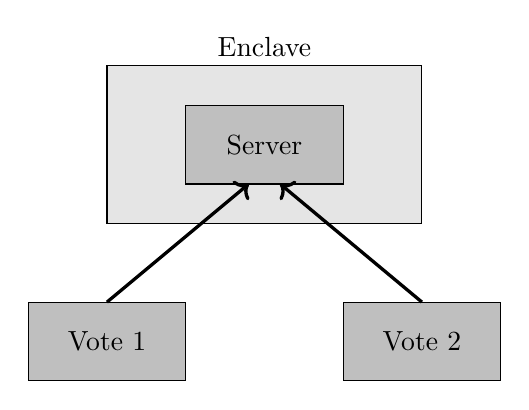
\begin{tikzpicture}
            \filldraw[fill=gray!50, draw=black] (0,0) rectangle (2, 1) node[pos=.5] {Vote 1};
            \filldraw[fill=gray!50, draw=black] (4,0) rectangle (6, 1) node[pos=.5] {Vote 2};
            \filldraw[fill=gray!20, draw=black] (1,2) rectangle (5, 4);
            \node[above] at(3,4) {Enclave};
            \filldraw[fill=gray!50, draw=black] (2,2.5) rectangle (4, 3.5) node[pos=.5] {Server};
            \draw[->, line width=1.2pt] (1,1) -- (2.8,2.5);
            \draw[->, line width=1.2pt] (5,1) -- (3.2,2.5);
        \end{tikzpicture}
        \caption{Structure of the E-Voting system}
        \label{fig:struct}
    \end{figure}

    \section{Implementing an E-Voting application}
    For both parts of the application there are already templates which help you get
    started, for the server there is the file \texttt{server.c}, this file
    can be compiled, signed and run by running \texttt{make server.enc}.
    For the vote application there is the file \texttt{vote.c}, this
    file can be compiled without OpenSGX by running: \texttt{make vote.run}.    

    Additionally there is a small library for UNIX pipes, make yourself familiar
    with the library by having a look at the header file (\texttt{libpipe.h}),
    which is in the root directory as well. This library is automatically
    compiled and linked to both the server and the vote application.

    Now you have all the prerequisites to start writing the E-Voting application,
    keep some things in mind:
    \begin{itemize}
        \item The vote application should only know the vote of the user
        \item The server application should not leak any information about the voting process, neither direct nor indirect
        \item Implement a simple authentication mechanism using an ID for each user
        \item Think about how and when to retrieve the result
        \item Think about how you can avoid side channel attacks, i.e. through timing measuremnts
        \item What is the problem of using named pipes?
    \end{itemize}

    \section{Attestation}
    Until now we assumed that the code that is being run in the enclave is the code that we wrote. To be sure that
    this is the case we now want to add attesation to our application. Both OpenSGX and Intel SGX support two
    forms of attestation: local and remote attestation, for this demonstration we will only implement local
    attestation, as all parts of the application run on the same machine. 

    For the attestation you will write a third program called \texttt{attest}, this program is required to run in
    an enclave as well. A template for this program is given in the file \texttt{attest.c}, the file can be run
    by typing \texttt{make attest.enc}. Think about how the voting procedure needs to be adapted to include local
    attestation, at which point should the user be able to verify the enclave?

    Have a look at the two examples provided by OpenSGX, they are located in the files 
    \texttt{opensgx/user/test/simple-remote-attest-challenger.c} and \\
    \texttt{opensgx/user/demo/simple-remote-attest-target.c}. Try to understand the
    examples and implement this mechanism as part of your application, the server will
    be the target and the attest application the challenger.


    \textbf{Good luck!}
\end{document}
